\documentclass [a4paper, 12pt]{article}

\usepackage[utf8]{inputenc}
\usepackage{amssymb}
\usepackage{amsmath}
\usepackage{bm}
\usepackage{epsfig}
\usepackage{graphicx}
\usepackage{times}
%\usepackage{placeins}
\usepackage{float}
\usepackage[usenames,dvipsnames]{xcolor}
\usepackage{caption}
\usepackage{subcaption}
\usepackage{hyperref}
\usepackage{cleveref}
\usepackage[version=4]{mhchem}
\usepackage{tikz}
\usetikzlibrary{decorations.markings}
\usetikzlibrary{shapes.misc,shapes.geometric,arrows,positioning,automata, patterns}


\textwidth 16 cm
\textheight 23 cm
\setlength{\oddsidemargin}{0.1 cm}
\setlength{\topmargin}{1 cm}
\setlength{\headheight}{0cm}
\setlength{\headsep}{0cm}
\setlength{\footskip}{0.75cm}
\setlength{\parindent}{0cm}
\setlength{\oddsidemargin}{0.1 cm}
\setlength{\itemsep}{10pt}
\bibliographystyle{gcs}

\DeclareUnicodeCharacter{2212}{-}
\newcommand{\matr}[1]{\bm{#1}}  

\begin{document}
 
\begin{figure}[H]
\begin{center}
  
\includegraphics[scale=0.45]{Figures/GCS-hlrs-fzj-lrz.jpg}\\
\end{center}
\end{figure}

\begin{center}
{\LARGE \bf Project Report} \\

\bigskip
\bigskip
\bigskip
\end{center}
\textbf{Period}\\
\phantom{MM}\textit{01.11.2017-26.04.2018}

\bigskip
\textbf{Project title}\\
\phantom{MM}\textit{KKRnano: Quantum description of skyrmions in chiral B20 magnets}

\bigskip
\textbf{Type of project}\\
\phantom{MM} \textit{new project}

%\bigskip
%\textbf{Project ID}\\
%\phantom{MM} \textit{Please provide in case of a project extension}

\bigskip
\textbf{Principal investigator}\\
\phantom{MM} \textit{ Prof. Dr. Stefan Bl{\"u}gel,
Institute for Advanced Simulation and Peter Gr\"unberg Institut, Forschungszentrum J\"ulich, D-52425 J\"ulich, Germany
}

\bigskip
\textbf{Project contributor(s)}\\

\phantom{MM} \textit{Marcel Bornemann,
Institute for Advanced Simulation and Peter Gr\"unberg Institut, Forschungszentrum J\"ulich, D-52425 J\"ulich, Germany
}

\phantom{MM} \textit{Dr. Sergii Grytsiuk,
Institute for Advanced Simulation and Peter Gr\"unberg Institut, Forschungszentrum J\"ulich, D-52425 J\"ulich, Germany
}

\phantom{MM} \textit{Dr. Roman Kováčik,
Institute for Advanced Simulation and Peter Gr\"unberg Institut, Forschungszentrum J\"ulich, D-52425 J\"ulich, Germany
}


\phantom{MM} \textit{Dr. Rudolf Zeller,
Institute for Advanced Simulation and Peter Gr\"unberg Institut, Forschungszentrum J\"ulich, D-52425 J\"ulich, Germany
}

\phantom{MM} \textit{Dr. Phivos Mavropoulos,
Institute for Advanced Simulation and Peter Gr\"unberg Institut, Forschungszentrum J\"ulich, D-52425 J\"ulich, Germany
}

%\phantom{MM} \textit{Dr. Paul F. Baumeister,
%Institute for Advanced Simulation and J\"ulich Supercomputing Centre, Forschungszentrum J\"ulich, D-52425 J\"ulich, Germany
%}


\newpage

\vfill
\tableofcontents
\vfill

\newpage

\begin{itemize}
	\item subject-specific results
	\item Performance on HazelHen
	\item typical job sizes
	\item Parallelization levels (OMP?)
	\item scaling behaviour \cite{brommel_juqueen_2017}
	\item runtimes
\end{itemize}

\section{Introduction}
We have developed a unique electronic structure code, 
KKRnano \cite{zeller_towards_2008,thiess_massively_2012},
specifically designed for petaFLOP computing. Our method scales linearly
with the number of atoms, so that we canrealize system sizes of up to 
half a million atoms in a unit cell if necessary.
\\
Recently, we implemented a relativistic generalization of our algorithm 
enabling us to calculate complex non-collinear magnetic structures, such as skyrmions,
in real space. Skyrmions are two-dimensional magnetization solitons, i.e. two-dimensional
magnetic structures localized in space, topologically protected by a non-trivial
magnetization texture, which has particle-like properties. 
\\
The focus of our work is on the germanide MnGe that is particularly
interesting among the chiral magnetic B20 compounds, as it exhibits a three-dimensional magnetic structure
that is not yet understood (see preliminary results
\cite{tanigaki_real-space_2015,rybakov_new_2016,bornemann_investigation_2017})


\section{Numerical Methods and Algorithms} 
%\rule{\textwidth}{0.4pt}\\
%\textit{Describe the numerical methods and algorithms that you are planning to use, improve, or develop.}\\
 
%\textit{(1 to 2 pages)}
%\bigskip

Contrary to other DFT codes, which determine the Kohn-Sham orbitals by solving
the Kohn-Sham differential wave equation, in KKRnano the Green function for the Kohn-Sham
equation is obtained by solving an integral equation in real space. For the solution, space is divided
into non-overlapping cells around the atoms, and the calculations are separated into single-cell parts
where only the potential within the individual cell enters, and a large complex linear matrix equation for 
the matrix elements $G_{LL}^{nn'} (\epsilon)$ of the Green function $G(r, r , \epsilon)$:
\begin{equation}
	G_{LL'}^{nn'} (\epsilon) = G_{LL'}^{r,nn'} (\epsilon) + \sum_{n''} \sum_{L''}
	G_{LL''}^{r,nn''} (\epsilon) \sum_{L'''} \Delta t_{L'' L'''}^{n''} (\epsilon)
	G_{L'''L'}^{n''n'} (\epsilon)
	\label{eq:dyson_eq}
\end{equation}
In the following we refer to $\Delta t_{L'' L'''}^{n''} (\epsilon)$ as the $\Delta t$-matrices and
$G_{LL''}^{r,nn''} (\epsilon)$ as the reference Green functions. We refer the reader to the existing
literature for more details \cite{zeller_towards_2008}.
\\
The given problem is identical to solving a complex linear matrix equation of the form
\begin{equation}
	\matr{A} \vec{x} = \vec{b}
\end{equation}
As is well known this problem scales as $O(N^3)$, where $N$ denotes the dimension of the $N \times N$
matrix $\matr{A}$. Standard solving schemes therefore severely limit the system size that can
be calculated.
However, by choosing a reference system of repulsive potentials
$\matr{A}$ can be made sparse and this can again be exploited
by using customized iterative algorithms for solving linear sparse matrix equations.
Our method uses the transpose free quasi minimal residual (TFQMR) algorithm \cite{freund_qmr:_1991}
which enables us to achieve $O(N^2)$ scaling. 
Convergence of the TFQMR iterations is achieved by working in the complex energy plane. Both concepts,
the repulsive reference system and application of complex energy, were
introduced by us into the KKR method \cite{zeller_application_1982,zeller_theory_1995}
and are used worldwide for many years. 
By truncating inter-atomic interactions above a certain distance, an $O(N)$ scaling 
behavior can be realized, and this feature should be used in any calculation involving more than 1000 atoms.
In most applications the TFQMR solver accounts for more than 70 \% of the computational work.
\\
For super-large-scale calculations (above 100000 atoms) the electrostatics solver begins
to require an amount of computing resources that is not negligible anymore. 
The electrostatic problem is given in terms of a Poisson equation that connects electric field and potential. 
Solving this equation scales quadratically with system size. 

\section{Scientific Results}

\begin{figure}[h]
\centering
\begin{subfigure}[b]{0.49\textwidth}
   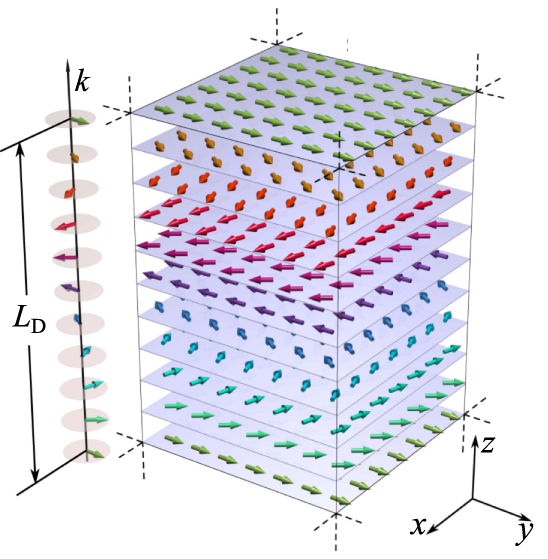
\includegraphics[width=\textwidth]{Figures/helicalspiral.png}
   \caption{}
   \label{fig:mnge_spiral}
\end{subfigure}
\begin{subfigure}[b]{0.49\textwidth}
	\includegraphics[width=\textwidth]{Figures/B20_hedgehog_antihedgehog.pdf}
   \caption{}
   \label{fig:mnge_3q}
\end{subfigure}
	\caption{Magnetic textures that are found experimentally in B20-\ce{MnGe}:  (a) Helical
	spin spiral that propagates in (001) direction. Figure is raken from \cite{rybakov_new_2016} b) 
	Magnetic anti-hedgehog texture that is wrapped around a magnetic monopole at the center. Figure is taken from \cite{zhang_electric_2016}.}
\label{fig:mnge_spiral_and_3q}
\end{figure}



Lately, special attention has been paid to cubic B20-type compounds with broken lattice inversion symmetry,
where skyrmion phases have been observed experimentally \cite{nagaosa_topological_2013}.
In a recent study \cite{tanigaki_real-space_2015} it was 
found by real-space observation transmission electron microscopy that a cubic lattice of skyrmionic hedgehogs
and anti-hedgehogs (see \Cref{fig:mnge_3q}) exists in B20-\ce{MnGe} 
with a lattice constant of about 3-6 nm.
Findings by Kanazawa et al. suggest that this lattice is set up by a superposition of three orthogonal
helical structures also referred to as 3Q state \cite{kanazawa_noncentrosymmetric_2017}. 
While the 3Q state certainly constitutes the most interesting non-trivial magnetic texture 
in B20-\ce{MnGe} there are also reports that the magnetic ground state in this system is
actually a helical spiral (see \Cref{fig:mnge_spiral}) \cite{yaouanc_magnetic_2017}.
These two observations are clearly contradictory and it was not yet explained how
both can be made within the same material.

Therefore, we performed
an analysis of these two helical states and the trivial ferromagnetic (FM) state.
The ferromagnet was identified as the ground state in the small unit cell (8 atoms), 
in which 1Q and 3Q state with their wavelengths of
3-6 nm do not fit.
\\
We begin by setting up a 6x6x6 B20-\ce{MnGe} supercell (1728 atoms), where we use PBEsol 
as exchange-correlation functional
and include only a single k-point, i.e. the $\gamma$-point.
In this initial comparison of ferromagnetic, 1Q and 3Q state using the equilibrium lattice constant
$a=4.80$ \AA \, the ferromagnet is predicted to be the ground state.
As this contradicts experimental observations we take into consideration that
in experiment the crystal structure might inadvertently differ from the ideal structure.
Such discrepancies can be caused e.g. by strain.
\\
Therefore, it is reasonable to check whether a material's properties change, when the
lattice constant is varied.
\begin{figure}[h]
\begin{center}
 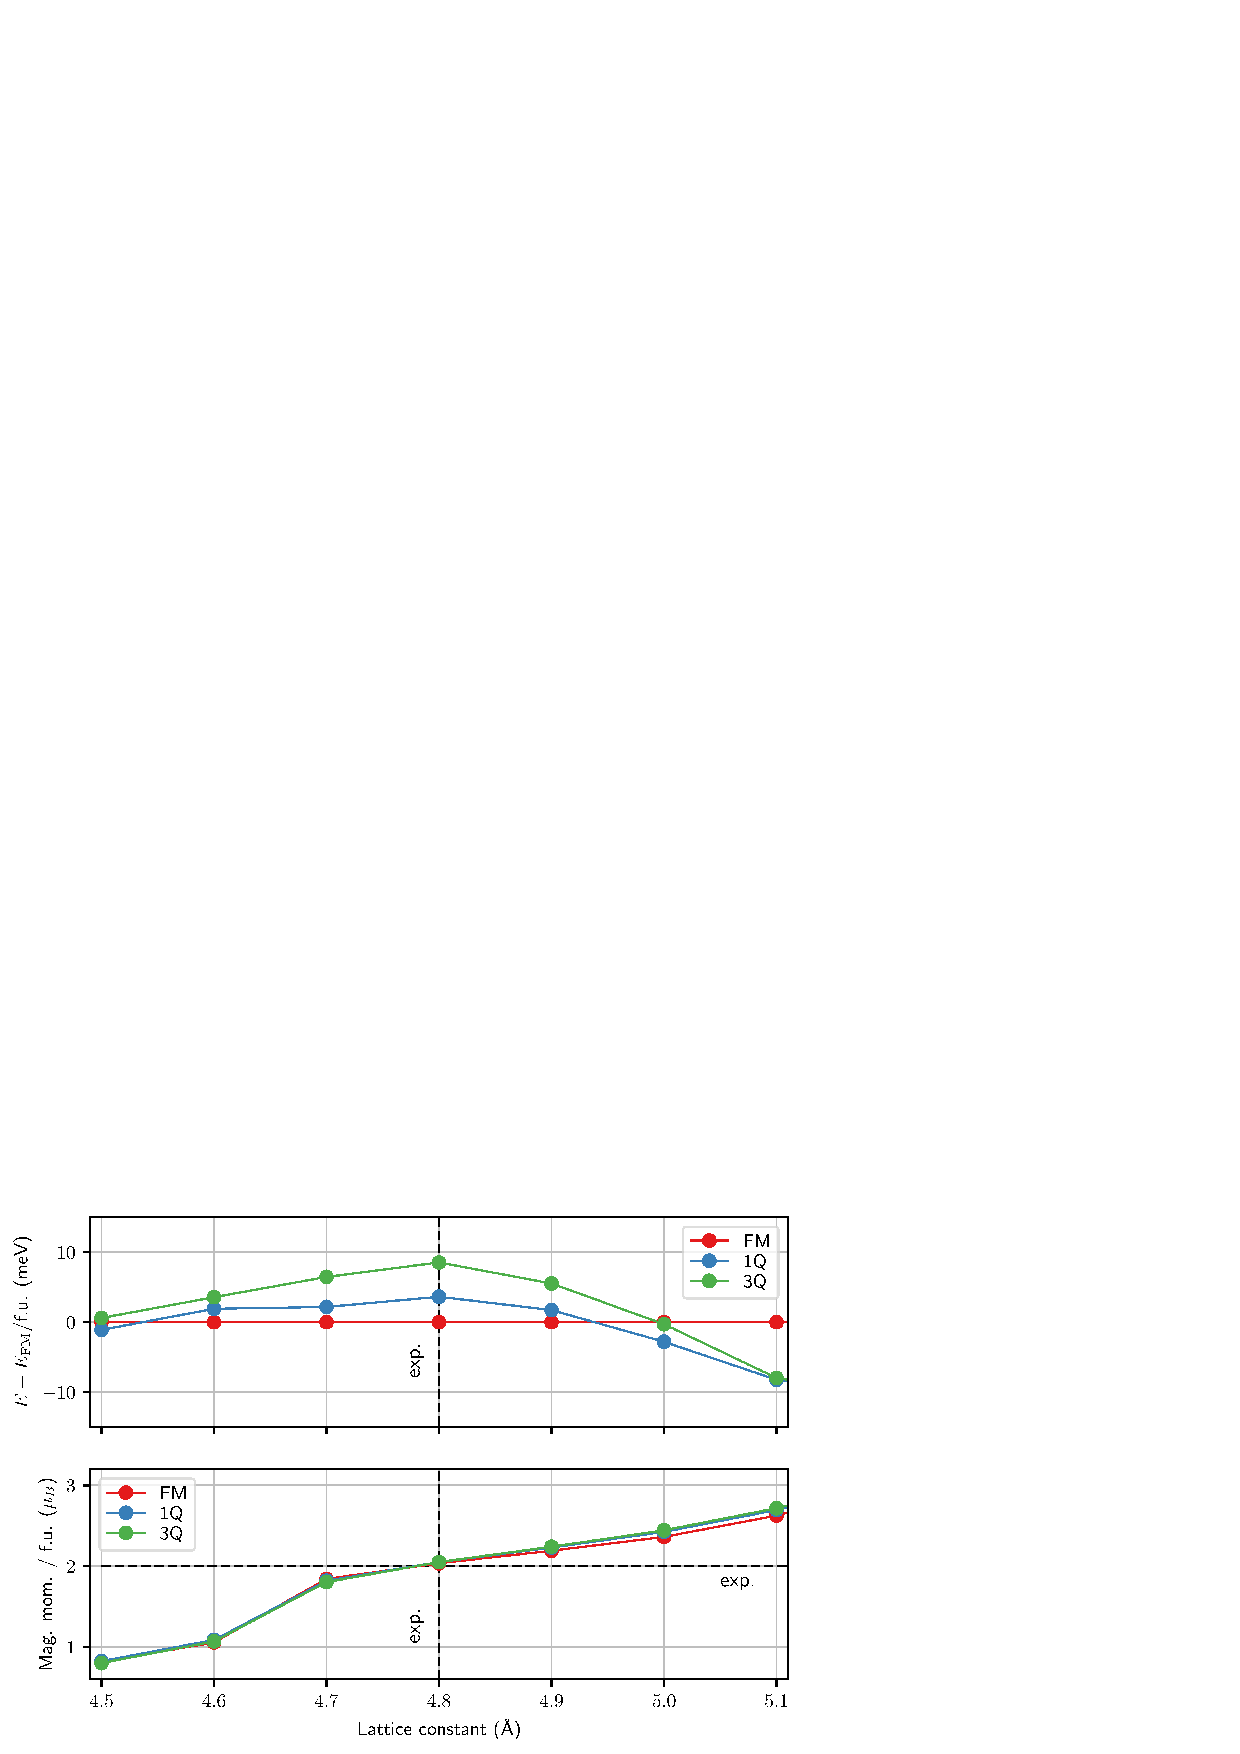
\includegraphics[width=\textwidth]{Figures/MnGe_ferro_1q.pdf}
\end{center}
\caption{
	Comparison of Ferromagnetic (FM), helical spiral (1Q) and hedgehog lattice (3Q) state with KKRnano.
	Top: Difference of total energies with the FM state as reference state for different lattice constants. 
	The experimental lattice constant is a = 4.80 \AA. 1Q and 3Q state are energetically preferrable 
	for $a > 5.0$ \AA. Bottom: Magnetic moment per Mn atom increases with lattice constant. 
	High-spin/Low-spin transition is clearly visible between a = 4.60 and a = 4.70 \AA.
	Experimentally, the magnetic moment is measured to be $\approx 2 \mu_{B}$.
	}
\label{fig:MnGe_ferro_1q}
\end{figure}
Such a variation is performed in the upper part of \Cref{fig:MnGe_ferro_1q}, where
the total energy is evaluated for FM, 1Q and 3Q state.
Clearly, neither the 1Q nor the 3Q state constitutes the ground state,
when the experimental lattice constant is assumed.
Yet, by increasing or decreasing the lattice constant the energetic difference can be made
smaller.
\\
We focus on an increase of the lattice constant rather than a decrease since 
the system goes into the low-spin state below $a=4.65$ \AA \, and according to experiment
the non-trivial textures
exist in the high-spin regime.
A crucial transition point is found around $a=5.0$ \AA,
where by imposing the 1Q or 3Q state the energy can be made smaller than for the ferromagnetic state.
In general, for $a>5.0$ \AA both helical states are favored over the ferromagnet.
\\
Obviously, an artifical increase of the lattice constant by
$0.2$ \AA \, ($\approx 4 \%$) or more is fairly large.
However, probes in experiment are seldom if ever perfectly clean and
impurities in the sample need to be considered as a source of error in the
final analysis. One potential
effect of impurities is chemical pressure that causes a spatial expansion of the
lattice structure.
An example of the possible effects of positive chemical pressure
can be found in \ce{Co}-doped B20-\ce{FeGe} \cite{stolt_chemical_2018}. 
Here, it was experimentally observed
that doping can increase the melting temperature and magnetic properties of a B20 alloy.
\\
In the lower part of \Cref{fig:MnGe_ferro_1q} the evolution of the magnetic moment
with decreasing/increasing lattice constant is tracked.
The resulting magnetic moment for the experimental lattice constant nicely falls 
on top of the magnetic moment of approximately $2 \mu_{B}$/f.u. 
which is reported by experimentalists \cite{yaouanc_magnetic_2017}.
\\
The high-spin/low-spin transition is recognizable between $a=4.60$ and $a=4.70$ \AA.
\\
Furhtermore, the magnetic moment increases, when the lattice constant is increased.
This is a common behaviour in DFT for metallic systems.
For larger lattice constants the magnetic moments of the three different
magnetic textures differ more than for the smaller lattice constants.
This could also give rise to the differences in the total energy.

\begin{itemize}
	\item Bloch point SOC scaling
\end{itemize}

%\FLoatBarrier
\section{Parallelization Scheme of KKRnano}
KKRnano features both MPI and OpenMP parallelization. The parallelization concept is sketched in
\Cref{fig:kkrnano_parallel}.
There are three MPI levels to parallelize over atoms,
spins and energy points. OpenMP is used in various parts of the code, mainly to parallelize important loops.
The single-site solver for calculations involving non-collinear magnetism
and the
TFQMR solver that solves the Dyson equation in \cref{eq:dyson_eq} 
are the parts that potentially benefit the most from OpenMP.

\begin{figure}[h!]
\centering
\begin{tikzpicture}[node distance=1cm]
%	\tikzstyle{process} = [rectangle, minimum width=3cm, minimum height=1cm, text centered, draw=black, fill=orange!30]
%	\tikzstyle{decision} = [diamond, minimum width=3cm, minimum height=1cm, text centered, draw=black, fill=green!30]
	\tikzstyle{serial_part} = [rectangle, rounded corners, minimum width=6cm, minimum height=1cm,text centered, draw=black]
	\tikzstyle{omp_part} = [rectangle, rounded corners, minimum width=6cm, minimum height=1cm,text centered, draw=black, fill=NavyBlue!40]
	\tikzstyle{omp_part2} = [rectangle, rounded corners, minimum width=6cm, minimum height=1cm,text centered, draw=black, pattern=north west lines, pattern color=NavyBlue!40]
%	\tikzstyle{io} = [trapezium, trapezium left angle=70, trapezium right angle=110, minimum width=3cm, minimum height=1cm, text centered, draw=black, fill=blue!30]
	\node (title1) [text centered, text width=6cm] {\textbf{Workflow in KKRnano}};
	\node (title2) [text centered, text width=6cm, right=of title1] {\textbf{MPI levels}};
	\node (ref) [omp_part2, below=of title1] {Set up reference system};
	\node (single) [omp_part, below=of ref] {Calculate single-site solutions};
	\node (dyson) [omp_part, below=of single] {Solve Dyson equation};
	\node (charge) [omp_part2, below=of dyson] {Calculate charge density};
	\node (pot) [omp_part2, below=of charge] {Calculate new potential};
	\node (mix) [omp_part2, below=of pot] {Mix potentials};

\draw [Black, very thick, ->] (ref.south) -- (single.north) ;
\draw [Black, very thick, ->] (single.south) -- (dyson.north) ;
\draw [Black, very thick, ->] (dyson.south) -- (charge.north) ;
\draw [Black, very thick, ->] (charge.south) -- (pot.north) ;
\draw [Black, very thick, ->] (pot.south) -- (mix.north) ;
	% MPI regions
	\def\AtomShift{8.25cm}
	\def\SpinShift{7.25cm}
	\def\EnergyShift{6.25cm}
	 \draw [Red, very thick, |-|] ([xshift=\AtomShift]ref.north) -- ([xshift=\AtomShift]mix.south) node [midway, rotate=90, fill=white, yshift=2pt] {Atoms} ;
	 \draw [Green, very thick, |-|] ([xshift=\SpinShift]ref.north) -- ([xshift=\SpinShift]mix.south) node [midway, rotate=90, fill=white, yshift=2pt] {Spins} ;
	 \draw [Orange, very thick, |-|] ([xshift=\EnergyShift]ref.north) -- ([xshift=\EnergyShift]dyson.south) node [midway, rotate=90, fill=white, yshift=2pt] {Energies} ;
	%	\draw[->, to path={-| (\tikztotarget)}]
%	  (ref) edge (mix) edge;
%	\node (dec1) [decision, below of=pro1, yshift=-0.5cm] {Decision 1};
%	\node (pro2a) [process, below of=dec1, yshift=-0.5cm] {Process 2a};
%	\node (pro2b) [process, right of=dec1, xshift=2cm] {Process 2b};
%	\node (out1) [io, below of=pro2a] {Output};
%	\node (stop) [startstop, below of=out1] {Stop};
\end{tikzpicture}
\caption{Schematic representation of MPI and OpenMP parallelization in KKRnano.
\\
The most important steps in the KKR workflow are depicted on the left side and the
three MPI regions over atoms, spins and energy points are indicated on the right side.
\\
Parts filled with blue comprise routines
where OpenMP is used and where this can be of high importance to the overall performance 
while in the striped blue parts
OpenMP is used but is less significant.
}
\label{fig:kkrnano_parallel}
\end{figure}


\subsubsection*{MPI parallelization over atoms}

The most crucial MPI level in KKRnano is the one for atoms since application scenarios for KKRnano
involve the treatment of a few thousand atoms and the KKR formalism allows us to solve the
multiple-scattering problem locally for each atom, if the Green functions of the reference system and
the t-matrices of the other scattering centers are provided (see \cref{eq:dyson_eq}).
In practice one MPI task handles 1-16 atoms.
\\
The reference Green functions are calculated by each task
for the atoms it is responsible for and are then sent to other tasks that require them. 
The reference t-matrices for the atoms inside the respective reference cluster are not communicated 
but calculated by each task individually as it takes less time to re-compute them than communicating them.
In any case the $\Delta t$-matrices of the actual systems need to be communicated.
After the necessary information is distributed, the Dyson equation can be solved independently by each task.
The calculation of the local charge density can also be conducted locally since only the diagonal
$nn$-elements are needed for this.
In order to subsequently obtain the potential from the local charge moments via the Poisson equation,
the moments must be shared with all other atom tasks by means of all-to-all communication.

\subsubsection*{MPI parallelization over spin channels}

If the system of interest is a collinear magnet, the two spin channels can be handled by two distinct
MPI tasks since the
magnetic Kohn-Sham equations are separable.
Due to the relatively small additional MPI communication effort
this yields an almost ideal speed-up by a factor of 2.
It should be noted that in the non-collinear KKR formalism such a 
separation of spin channels is no longer possible because 
there is intermixing and all operations involving the
$\Delta t$-matrices and Green functions in the global frame of reference
need to be performed in full spin space, i.e. $\{\uparrow \uparrow, \uparrow \downarrow,
\downarrow \uparrow, \downarrow \downarrow \}$.
Thus, the spin parallelization level can only be used in connection with
a collinear calculation.


\subsubsection*{MPI parallelization over energy points}

The requirement to calculate the Green function at different energy points offers another possibility to
introduce a parallel level since the values of the Green function $G(\vec{r},\vec{r},E_i)$ at energy points $E_i$
can be obtained in parallel.
After the values are obtained the results must be distributed among the processes within
the energy parallelization level to recover the full Green function at all energy points.
\\
Assigning one MPI task to each energy point is not a promising concept because
of the significantly different runtimes per energy point. Especially the points closest to the
Fermi level (and therefore to the real axis)
need many more k-points and TFQMR iterations than the points that lay high up in the complex plane (see
\cref{fig:energy_contour}).
Therefore the energy points are split into three different groups and each group is taken care of by
one MPI task. In the first iteration of the self-consistency cycle the points are equally distributed to all
groups. At the end of the first iteration the points are regrouped depending on how much time the iteration took
for each point. The aim is to find a grouping for which all groups of energy points are converged at
a similar time so that idling is avoided. This is also referred to as \textit{dynamical load-balancing}.
A correct load-balancing is of outmost importance to the effectiveness of this MPI level since
all tasks need to have finished before the program can move on to the solution of the electrostatic problem,
i.e. the Poisson equation.
Due to the challenge that load-balancing can pose, parallelization over energy points should only be used, 
if plenty of processor cores are available and
ought to be utilized.
\\
A lookahead on the performance results presented in \cref{sec:benchmarks_bgq}
reveils that with growing system size
the electrostatic problem, which in terms of energy parallelization
must be considered a serial part of the code, becomes computationally more releveant.
\Cref{kkrnano:mnge_weakscaling_moderateomp} shows 
that the fraction of the electrostatics (ES) solver runtime compared to the combined runtime
of TFQMR solver and ES solver
ranges from $\alpha=\frac{84}{432+84}=0.16$ for 8,192 atoms to $\alpha=\frac{470}{430+470}=0.52$ for
229,736 atoms.
According to \cref{eq:amdahl_limit} this limits the maximum speedup that can be achieved
by energy parallelization to $S_{r} \rightarrow 6.25$ and $S_{r} \rightarrow 1.92$, respectively.



\subsubsection*{OpenMP parallelization}

KKRnano can be compiled either with or without support for OpenMP. If it is enabled,
loops primarily in the TFQMR solver but also in the routines that calculate the regular and irregular
solutions are executed using parallel threads. 
This is particularly useful on architectures that support simultaneous multithreading (SMT).
However, we try to use BLAS (Basic Linear Algebra Subprograms) library routines for arithmetic
operations, e.g. matrix-matrix multiplications, throughout our code. BLAS libraries usually
have their own built-in SMT support.
Therefore, the available SMT threads must be partitioned between the explicit OpenMP 
parallel regions in the code and the implicit parallelization of the BLAS library.
Here, the optimal partitioning is highly architecture-dependent and a general recommendation cannot
be given.


\subsubsection*{Multiple Atoms per Thread}

Assigning multiple atoms to one MPI task is beneficial, if very large systems are
supposed to be calculated on a comparatively small allocation of compute nodes.
\\
KKRnano can treat multiple atoms per atomic MPI task by using the following algebraic scheme: 
We rewrite the Dyson equation from \cref{eq:dyson_equation_lap} which reads
\beq
\sum_{\mu} \sum_{L'} A^{\nu \mu}_{LL'} X^{\mu}_{L'L''} = b_{L'L''}
\eeq
where $\nu$ and $\mu$ indicate atomic positions and the indices $L$,$L'$ and $L''$ denote
the appropriate expansion in angular momentum components. $A$ has dimension 
$N_{\text{cl}} (l_{\text{max}}+1)^2 \times N_{\text{tr}} (l_{\text{max}}+1)^2$,
$b$ usually has the
negative local $\Delta t$ as diagonal elements
and $X$ has dimension $N_{\text{cl}} (l_{\text{max}}+1)^2 \times (l_{\text{max}}+1)^2$.
$A$ is a matrix of blocks of size ${(l_{\text{max}}+1)}^2 \times {(l_{\text{max}}+1)}^2$
while $X$ and $b$ are vectors
of such blocks. For more than a single atom per task $x$ and $b$ can also take a matrix form
with dimension $N_{\text{cl}} (l_{\text{max}}+1)^2 \times N_{\text{loc}} (l_{\text{max}}+1)^2$, where
$N_{\text{loc}}$ is the number of atoms treated by one MPI task of the atom parallelization level.
The corresponding linear equation system reads
\beq
\label{eq:dyson_equation_lap_multi}
\sum_{\mu} \sum_{L'} A^{\nu \mu}_{LL'} X^{\mu \gamma}_{L'L''} = b_{L'L''}
\eeq
, where an additional index $\gamma$ is introduced that runs over $N_{\text{loc}}$. 

\section{Benchmark Results on HazelHen}

\begin{itemize}
	\item Benchmarks for 6,8,10,12,18,24 MnGe
	\item Potentially benchmarks for larger systems obtained during the workshop at HLRS
	\item 50 iterations in each run leads to approx. 8 hours of walltime
	\item Total runtimes and time consumption of multiple-scattering and other important routines
\end{itemize}

\newpage

\bibliography{My_Library}

%\section{Bibliographic References}
%\rule{\textwidth}{0.4pt}\\
%\textit{Provide recent/most important bibliographic references that are relevant to the project.}\\

\bigskip
\begin{flushright}
{\tiny V1.3-2016JUN07}
\end{flushright}
\end{document}
